\IfFileExists{siamart220329.cls}
  {\documentclass[final,leqno]{siamart220329}}
  {\documentclass[11pt,twocolumn]{article}}

\usepackage{amsmath,amssymb,amsthm,mathtools}
\usepackage{booktabs}
\usepackage{enumitem}
\usepackage{microtype}
\usepackage{xcolor}
\usepackage{tikz}
\usetikzlibrary{arrows.meta,calc,positioning}
\usepackage[hidelinks]{hyperref}
\setlength{\emergencystretch}{2em}

\definecolor{dgray}{RGB}{70,70,80}
\definecolor{dblue}{RGB}{28,82,150}
\definecolor{dred}{RGB}{155,45,45}
\definecolor{dgold}{RGB}{170,125,35}
\definecolor{dgreen}{RGB}{35,125,85}
\tikzset{
  prim/.style={dgray,thick},
  hlt/.style={dblue,very thick},
  deg/.style={dred,thick},
  gold/.style={dgold,very thick},
  greenline/.style={dgreen,very thick},
  faint/.style={dgray!35,thin},
  ann/.style={dgray,font=\scriptsize},
  box/.style={draw=dgray!70,rounded corners=2pt,inner sep=3pt,align=center,font=\scriptsize},
  arrow/.style={-{Latex[length=2.2mm]},thick,dgray}
}

\makeatletter
\@ifclassloaded{article}{%
  \usepackage[letterpaper,margin=0.72in,columnsep=0.25in]{geometry}
  \setlength{\parindent}{1em}
  \setlength{\parskip}{0pt}
}{}
\@ifundefined{headers}{\newcommand{\headers}[2]{}}{}
\@ifundefined{keywords}{%
  \newenvironment{keywords}{\par\smallskip\noindent\textbf{Key words.}}{\par}
}{}
\@ifundefined{AMS}{%
  \newenvironment{AMS}{\par\smallskip\noindent\textbf{AMS subject classifications.}}{\par}
}{}
\makeatother

\setlist{leftmargin=*,itemsep=1pt,topsep=2pt}
\allowdisplaybreaks

\DeclareMathOperator{\diag}{diag}
\DeclareMathOperator{\dist}{dist}
\DeclareMathOperator{\rank}{rank}
\DeclareMathOperator{\spec}{spec}
\DeclareMathOperator{\cond}{cond}
\newcommand{\C}{\mathbb{C}}
\newcommand{\R}{\mathbb{R}}
\newcommand{\T}{\mathbb{T}}
\newcommand{\N}{\mathbb{N}}
\newcommand{\eps}{\varepsilon}
\newcommand{\dd}{\,d}
\newcommand{\pv}{\operatorname{p.v.}}
\newcommand{\one}{\mathbf{1}}
\newcommand{\wh}{\widehat}
\newcommand{\norm}[1]{\left\lVert #1\right\rVert}
\newcommand{\ip}[2]{\left\langle #1,#2\right\rangle}

\makeatletter
\@ifundefined{theorem}{\newtheorem{theorem}{Theorem}[section]}{}
\@ifundefined{proposition}{\newtheorem{proposition}[theorem]{Proposition}}{}
\@ifundefined{lemma}{\newtheorem{lemma}[theorem]{Lemma}}{}
\@ifundefined{corollary}{\newtheorem{corollary}[theorem]{Corollary}}{}
\@ifundefined{definition}{\theoremstyle{definition}\newtheorem{definition}[theorem]{Definition}}{}
\@ifundefined{remark}{\theoremstyle{remark}\newtheorem{remark}[theorem]{Remark}}{}
\makeatother

\title{The Log-Discriminant Hessian for Near-Boundary Quadrature}
\author{Rick Gulati\thanks{BlueChips Research and The Wharton School,
University of Pennsylvania, Philadelphia, PA 19104, USA
(\texttt{rkgulati@wharton.upenn.edu}).}}
\headers{The Log-Discriminant Hessian for Near-Boundary Quadrature}{R. Gulati}

\begin{document}
\maketitle

\begin{abstract}
We study a polynomial-algebraic discretization of the hypersingular
boundary operator that controls near-boundary layer-potential
quadrature.  For distinct points
$V=(v_1,\ldots,v_n)\subset\C$ let
\[
  \begin{aligned}
  \Delta(V)&=\prod_{i<j}(v_i-v_j)^2,\\
  Q(V)&=-\tfrac12\nabla_V^2\log|\Delta(V)|.
  \end{aligned}
\]
In complex coordinates this Hessian is the chord-squared graph
Laplacian
\[
  \begin{aligned}
  Q_{ij}&=-|v_i-v_j|^{-2}\quad (i\ne j),\\
  Q_{ii}&=\sum_{k\ne i}|v_i-v_k|^{-2}.
  \end{aligned}
\]
On the regular $n$-gon it is circulant and has the exact spectrum
$\lambda_m=m(n-m)/2$, $m=0,\ldots,n-1$.  After multiplication by the
arclength weight this spectrum converges to that of
$\pi(-\Delta_{S^1})^{1/2}$, and on a $C^3$ closed curve the continuum
operator
\[
 (Q_\Gamma f)(s)=\pv\int_\Gamma
 \frac{f(s)-f(t)}{|\gamma(s)-\gamma(t)|^2}\dd t
\]
satisfies $Q_\Gamma=\pi\Lambda_\Gamma+K_0$, where
$\Lambda_\Gamma$ is the Dirichlet-to-Neumann map and
$K_0\in\Psi^0(\Gamma)$.  This gives an intrinsic explanation of the
$n\delta\sim1$ breakdown threshold for the periodic trapezoidal rule
near a boundary: the error splits into a bulk analytic-continuation
channel and a local channel with universal profile
$\operatorname{Re}\log(1-e^{-2\pi\rho+2\pi i\beta})$,
$\rho=\delta/h$.  The same operator yields an $O(n\log n)$ functional
calculus on the circle, an $O(n)$-conditioned hypersingular
discretization modulo lower order terms, and a minimax quadrature
rate on analytic Jordan curves governed by the sum of the density
collar modulus and the target conformal distance.
\end{abstract}

\begin{keywords}
near-singular quadrature, layer potentials, hypersingular boundary
integral equations, Dirichlet-to-Neumann map, discriminant, Fekete
points, periodic trapezoidal rule
\end{keywords}

\begin{AMS}
65D32, 65N38, 65T50, 31A10, 35S05
\end{AMS}

\section{Introduction}

Layer potentials give high-order solvers for planar boundary value
problems, but their direct quadrature becomes delicate when the target
approaches the source curve.  For a smooth closed curve
$\Gamma\subset\C$ and a density $\sigma$ consider
\begin{equation}\label{eq:intro-layer}
  I(x)=\int_\Gamma \log|x-y|\,\sigma(y)\dd s(y),\qquad x\notin\Gamma.
\end{equation}
The periodic trapezoidal rule is exponentially accurate when the
target is separated from $\Gamma$ by a distance large compared with
the mesh width \cite{TW2014}.  As soon as the normal distance
$\delta=\dist(x,\Gamma)$ becomes comparable with the spacing
$h=L/n$, the logarithmic kernel has a singularity within one mesh
cell of the contour and the error no longer follows the resolved
analytic rate.  This is the near-singular quadrature problem addressed
by specialized methods such as panel refinement, singularity
subtraction, and quadrature by expansion \cite{HelsingOjala2008,
Kloeckner2013,KlintebergTornberg2017}.

There are two scales in this failure.  The first is analytic: the
classical trapezoidal estimate is controlled by how far the integrand
can be continued off the real parameter axis before meeting a
singularity.  The second is discrete and local: when the nearest
complex singularity lies within $O(h)$ of a node, the error is set by
the unresolved tangent-line logarithm rather than by the global
analytic strip.  The numerical literature handles the second scale
very effectively by changing the quadrature rule.  The purpose here is
different: identify the boundary operator whose spectrum and symbol
explain why the second scale is intrinsic.

This paper isolates a single operator behind that transition.  It is
not introduced by regularizing the singular integral.  It is the
Hessian of the logarithm of a polynomial discriminant.  The resulting
matrix is a weighted graph Laplacian with weights
$|v_i-v_j|^{-2}$, and on roots of unity it has a closed form Fourier
spectrum.  The continuum limit is the principal part of the
hypersingular boundary integral operator, equivalently the
Dirichlet-to-Neumann map up to the factor $\pi$ and a bounded
zeroth-order remainder.

The main contributions are as follows.
\begin{enumerate}
\item The discrete log-discriminant Hessian $Q_n$ on the regular
$n$-gon has eigenvalues $m(n-m)/2$.  Its weighted continuum scaling
has symbol $\pi|\xi|$, giving an FFT functional calculus at
$O(n\log n)$ cost.
\item On a $C^3$ curve, the continuum inverse-square operator
$Q_\Gamma$ equals $\pi\Lambda_\Gamma$ modulo $\Psi^0$.  Therefore
the chord-squared discretization is a direct Nyström discretization
of the hypersingular operator's order-one part.
\item The trapezoidal error near $\Gamma$ has a two-channel
decomposition: a bulk channel controlled by analytic continuation
and a local channel controlled by the universal profile
\[
  \mathcal M(\rho,\beta)
   =\operatorname{Re}\log(1-e^{-2\pi\rho+2\pi i\beta}),
  \qquad \rho=\delta/h.
\]
The crossover occurs at $\rho=O(1)$, i.e., $n\delta/L=O(1)$.
\item On analytic Jordan curves the minimax error over Hardy-class
densities has exponential rate
\[
  n^{-1}\exp\!\left[-\frac n2
   \bigl(\log\rho+\delta_\Phi(x)\bigr)\right],
\]
where $\log\rho$ is the density collar width and
$\delta_\Phi(x)$ is the exterior conformal distance of the target.
\end{enumerate}
Longer geometric material from the source manuscript, including the
discriminant-cone interpretation and inverse-spectral pipeline, is
not used in the proofs below and is omitted from this SIAM-length
version.

The organization follows the chain from algebra to numerics.  Section
2 derives the log-discriminant Hessian and its exact polygon spectrum,
including the spectral-renormalization identity that explains why
logarithmic coordinates and zeta tails appear.  Section 3 passes to
smooth curves and identifies the continuum operator with the
Dirichlet-to-Neumann map modulo lower order terms.  Section 4 proves
the near-singular bridge and separates the bulk and local error
channels.  Section 5 states the analytic minimax rate in conformal
coordinates.  Section 6 gives the reduced numerical evidence, and
Section 7 records the geometric reading and limitations.

\section{The Algebraic Operator}

Let $V=(v_1,\ldots,v_n)$ be a configuration of distinct complex
points.  The discriminant
\[
  \Delta(V)=\prod_{1\le i<j\le n}(v_i-v_j)^2
\]
vanishes precisely on collisions.  On the collision-free
configuration space the function
\[
  \Phi(V)=\log|\Delta(V)|=2\sum_{i<j}\log|v_i-v_j|
\]
is real analytic.  Its negative half Hessian is the matrix
\begin{equation}\label{eq:Q-def}
  Q_{ij}(V)=
  \begin{cases}
  -|v_i-v_j|^{-2},& i\ne j,\\[2mm]
  \displaystyle\sum_{k\ne i}|v_i-v_k|^{-2},& i=j.
  \end{cases}
\end{equation}
The identity follows by differentiating each two-point logarithm in
complex coordinates.  The row sums vanish and the quadratic form is
\begin{equation}\label{eq:Q-form}
  u^*Q(V)u
   =\frac12\sum_{i\ne j}\frac{|u_i-u_j|^2}{|v_i-v_j|^2}.
\end{equation}
Thus $Q(V)$ is positive semidefinite and has kernel exactly the
constant vector when the interaction graph is connected.

\subsection{Log-Hessian identity}

The definition is coordinate-free enough for the present purposes, but
the elementary calculation is worth recording because it fixes the
normalization.  Write a complex point as $v=x+iy$.  For $i\ne j$,
\[
  \nabla_{v_i}\nabla_{v_j}\log|v_i-v_j|
\]
has the real $2\times2$ block of the Coulomb Hessian.  When the
normal/tangential degrees of freedom are compressed onto scalar
boundary data, the mixed scalar block is $-|v_i-v_j|^{-2}$.  Summing
the pair interactions over all unordered pairs gives the diagonal
completion in \eqref{eq:Q-def}.  Equivalently, for scalar variations
$u=(u_1,\ldots,u_n)$,
\[
  \begin{aligned}
  -\frac12\frac{\dd^2}{\dd\eps^2}
  \Phi(&v_1+\eps u_1,\ldots,v_n+\eps u_n)\bigg|_{\eps=0}\\
  &=
  \frac12\sum_{i\ne j}\frac{|u_i-u_j|^2}{|v_i-v_j|^2},
  \end{aligned}
\]
after taking the boundary scalar component of the variation.  This is
why the Hessian is a Laplacian rather than a general dense symmetric
matrix.

Three invariances are immediate.  Translation of all $v_i$ leaves
$Q(V)$ unchanged.  Rotation and dilation by $a\in\C^\times$ multiply
the weights by $|a|^{-2}$.  Relabeling nodes conjugates the matrix by
the corresponding permutation.  These invariances are exactly the
similarity invariances expected of the principal part of a boundary
operator.

\subsection{The regular polygon}

Set $\omega=e^{2\pi i/n}$ and
$V_\omega=(1,\omega,\ldots,\omega^{n-1})$.  The corresponding matrix
$Q_n:=Q(V_\omega)$ is circulant.  Its first row is
\[
  \begin{aligned}
  (Q_n)_{00}&=\sum_{k=1}^{n-1}\frac1{|1-\omega^k|^2},\\
  (Q_n)_{0k}&=-\frac1{|1-\omega^k|^2}\quad(k\ne0).
  \end{aligned}
\]

\begin{theorem}[polygon spectrum]\label{thm:polygon-spectrum}
For $m=0,\ldots,n-1$, the Fourier mode
$\varphi_m(j)=n^{-1/2}\omega^{mj}$ is an eigenvector of $Q_n$ with
\begin{equation}\label{eq:spectrum}
  \lambda_m(Q_n)=\frac{m(n-m)}2.
\end{equation}
Consequently $\ker Q_n=\operatorname{span}\{\one\}$ and
$\cond(Q_n|_{\one^\perp})=O(n)$.
\end{theorem}

\begin{proof}
For a circulant graph Laplacian the eigenvalue on mode $m$ is
\[
  \lambda_m=\sum_{k=1}^{n-1}
  \frac{1-\omega^{mk}}{|1-\omega^k|^2}.
\]
The imaginary part cancels by pairing $k$ and $n-k$.  The real part
is
\[
  \frac12\sum_{k=1}^{n-1}
  \frac{2-\omega^{mk}-\omega^{-mk}}
       {(1-\omega^k)(1-\omega^{-k})}.
\]
Using
\[
 \frac{1-z^m}{1-z}=1+z+\cdots+z^{m-1},\qquad z=\omega^k,
\]
the summand becomes one half of a finite geometric convolution.
Orthogonality of the nontrivial roots of unity leaves exactly the
$m(n-m)$ surviving pairs.  This gives \eqref{eq:spectrum}.
\end{proof}

The arclength-weighted matrix
\begin{equation}\label{eq:weighted-Q}
  \mathsf Q_n=\frac{2\pi}{n}Q_n
\end{equation}
has eigenvalues $\pi m(1-m/n)$ for $0\le m\le n-1$.  For fixed
Fourier index $m$ and $n\to\infty$ this converges to $\pi|m|$, the
spectrum of $\pi(-\Delta_{S^1})^{1/2}$.

\begin{corollary}[functional calculus]\label{cor:fcalc}
Let $\varphi$ be defined on $\spec(Q_n)$.  If $F_n$ is the unitary
DFT, then
\[
  \varphi(Q_n)u
   =F_n^*\diag\!\bigl(\varphi(m(n-m)/2)\bigr)_{m=0}^{n-1}F_nu .
\]
Each application costs $O(n\log n)$.  On $\one^\perp$ this gives
fast inverses, fractional powers, heat semigroups, and spectral
filters.
\end{corollary}

\begin{remark}
The null flux identity $Q_n\one=0$ is algebraic.  It is not a
quadrature accident and does not depend on cancellation at machine
precision.  This matters for hypersingular equations, where failure
to preserve the constant nullspace produces visible flux leakage.
\end{remark}

\subsection{Cauchy--Gram factorization}

The spectrum in Theorem~\ref{thm:polygon-spectrum} can also be read
as a Cauchy--Gram identity.  Let $p(z)=z^n-1$ and write
\[
  \frac{p'(z)}{p(z)}
  =\sum_{j=0}^{n-1}\frac1{z-\omega^j}.
\]
Taking boundary traces on the roots and subtracting the singular
self-term produces the same inverse chord weights as \eqref{eq:Q-def}.
In Fourier variables, multiplication by $z^m$ and the root identities
\[
  \sum_{j=0}^{n-1}\omega^{j\ell}=
  \begin{cases}
  n,& \ell\equiv0\pmod n,\\
  0,& \text{otherwise}
  \end{cases}
\]
leave only the pairs $(a,b)$ with $0\le a<m$ and
$m\le b<n$.  Their number is $m(n-m)$, and the factor $1/2$ is the
symmetrization between the two endpoints of the chord.  This is the
finite-dimensional form of the Cauchy projection identity behind the
half-Laplacian on the circle.

\subsection{Spectral renormalization}

The quadratic spectrum $m(n-m)/2$ contains a bulk term and two
boundary tails.  This decomposition is useful because it is the same
bulk/local splitting that reappears in the quadrature bridge.  Define
\begin{equation}\label{eq:Sn}
  S_n(s)=\sum_{m=1}^{n-1}
  \left(\frac{m(n-m)}{n}\right)^{-s}.
\end{equation}
For $\operatorname{Re}s<1$ the corresponding bulk integral is
$n^{1-s}B(1-s,1-s)$; both sides then extend meromorphically.

\begin{theorem}[renormalized spectral tail]\label{thm:zeta-tail}
Let
\[
  T_n(s)=S_n(s)-n^{1-s}B(1-s,1-s).
\]
For every compact $K\subset\C\setminus\mathbb Z_{\ge1}$ there is
$C_K$ such that
\begin{equation}\label{eq:zeta-tail}
  |T_n(s)-2\zeta(s)|\le C_K n^{-1},
  \qquad s\in K,\quad n\ge2.
\end{equation}
In particular $T_n(0)=-1=2\zeta(0)$.
\end{theorem}

\begin{proof}[Proof sketch]
Apply Euler--Maclaurin to
$f_s(x)=(x(1-x))^{-s}$ on $[1/n,1-1/n]$ after cutting off the two
endpoints.  The interior contribution is
$n^{1-s}B(1-s,1-s)$, while the two endpoint tails are
\[
  \sum_{m\ge1}m^{-s}+ \sum_{m\ge1}m^{-s}=2\zeta(s)
\]
after analytic continuation.  The matching terms at the cutoffs
cancel between the bulk integral and the truncated tails.  Uniformity
on compact subsets away from the positive integers follows either
from the Euler--Maclaurin remainder with a fixed number of endpoint
subtractions or from the Mellin--Barnes contour representation of
$(1-x)^{-s}$.  The direct identity at $s=0$ is
$(n-1)-n=-1$.
\end{proof}

The theorem says that the zeta function is not an extra analytic
object added to the polynomial calculation; it is the residual
boundary tail of the finite discriminant spectrum after the unique
bulk counterterm has been removed.  This is also why logarithms rather
than powers are the natural coordinates in the near-boundary estimates:
multiplicative collars become additive distances after the Mellin
renormalization.

\section{Continuum Limit and Hypersingular Operators}

Let $\Gamma$ be a closed $C^3$ Jordan curve parametrized by arclength
$\gamma:\R/L\mathbb Z\to\C$.  Define
\begin{equation}\label{eq:Q-cont}
  (Q_\Gamma f)(s)=\pv\int_0^L
  \frac{f(s)-f(t)}{|\gamma(s)-\gamma(t)|^2}\dd t .
\end{equation}
The principal singularity is the one-dimensional inverse-square
kernel.  Since
$|\gamma(s)-\gamma(t)|^2=(s-t)^2+O(|s-t|^4)$, the local model is
\[
  \pv\int_\R \frac{f(s)-f(t)}{(s-t)^2}\dd t=\pi |D|f(s).
\]
The curvature-dependent difference is less singular.

\begin{lemma}[tangent-graph decomposition]\label{lem:tangent}
In every sufficiently small arclength chart,
\begin{equation}\label{eq:tangent-decomp}
  \frac{1}{|\gamma(s)-\gamma(t)|^2}
  =
  \frac{1}{(s-t)^2}+b_0(s,t),
\end{equation}
where $b_0$ is locally integrable as a finite-part kernel and defines
a pseudodifferential contribution of order $0$.  More precisely, if
$\gamma\in C^3$, then after subtracting the tangent-line kernel the
remaining operator maps $H^{1/2}$ to $H^{1/2}$ locally.
\end{lemma}

\begin{proof}
Taylor expansion in arclength gives
\[
 \begin{aligned}
 \gamma(t)=\gamma(s)&+(t-s)T(s)\\
 &+\tfrac12(t-s)^2\kappa(s)N(s)+O(|t-s|^3).
 \end{aligned}
\]
Because $T\cdot N=0$ and $|T|=1$,
\[
 |\gamma(t)-\gamma(s)|^2
 =(t-s)^2-\frac{\kappa(s)^2}{12}(t-s)^4+O(|t-s|^5).
\]
Therefore the difference between the reciprocal chord square and
$(s-t)^{-2}$ is bounded at the diagonal up to the finite smoothness
allowed by $\gamma$.  The off-diagonal part is smooth, so the induced
operator has order zero.
\end{proof}

\begin{theorem}[Dirichlet-to-Neumann identification]\label{thm:dtn}
On mean-zero functions on a $C^3$ closed curve,
\begin{equation}\label{eq:dtn}
  Q_\Gamma=\pi\Lambda_\Gamma+K_0,
\end{equation}
where $\Lambda_\Gamma$ is the interior Dirichlet-to-Neumann map and
$K_0\in\Psi^0(\Gamma)$.  In particular $Q_\Gamma$ is an elliptic
order-one pseudodifferential operator with principal symbol
$\pi|\xi|$.
\end{theorem}

\begin{proof}
Work in an arclength chart near $s=t$.  Taylor expansion gives
\[
  \frac1{|\gamma(s)-\gamma(t)|^2}
   =\frac1{(s-t)^2}+a_0(s,t),
\]
where $a_0$ is a conormal kernel of order $0$ under the stated
regularity.  The first term has Fourier multiplier $\pi|\xi|$.  The
Dirichlet-to-Neumann map has principal symbol $|\xi|$
\cite{Hormander1985,McLean2000}.  Patching the local charts by a
partition of unity leaves a global zeroth-order remainder.
\end{proof}

\begin{remark}[what the theorem does and does not say]
The identity \eqref{eq:dtn} is a principal-symbol statement with a
controlled lower-order remainder.  It does not claim that the chord
kernel is a new formula for the full Dirichlet-to-Neumann map on an
arbitrary curve.  It says that the algebraic Hessian selects the
canonical order-one part of that map without choosing a regularization
of a hypersingular integral.
\end{remark}

\begin{proposition}[rigidity on the circle]\label{prop:rigidity}
On $S^1$, suppose $A$ is a real, translation-invariant,
positive-semidefinite operator on mean-zero trigonometric polynomials
whose quadratic form is invariant under rotations, has order-one
homogeneity under dilation of the boundary length, and agrees with the
two-point inverse-square interaction on localized differences.  Then
$A=c|D|$ for some $c>0$.  With the normalization of
\eqref{eq:Q-cont}, $c=\pi$.
\end{proposition}

\begin{proof}
Translation invariance diagonalizes $A$ in the Fourier basis.  Reality
and reflection symmetry force the multiplier to depend only on
$|m|$.  Order-one homogeneity and positivity give a nonnegative
multiple of $|m|$ as the principal multiplier.  The inverse-square
normalization fixes the constant by the finite-part identity
\[
  \pv\int_\R \frac{1-e^{i\xi t}}{t^2}\dd t=\pi|\xi|.
\]
\end{proof}

\subsection{Nyström form}

For nodes $s_i$ with quadrature weights $w_i$ define
\begin{equation}\label{eq:nystrom}
  (Q_{\Gamma,n}u)_i
   =\sum_{j\ne i}w_j\,
    \frac{u_i-u_j}{|\gamma(s_i)-\gamma(s_j)|^2}.
\end{equation}
On the circle with equispaced nodes this is exactly
$(2\pi/n)Q_n$.  On smooth curves it is a direct discretization of
the order-one part of the Hadamard finite-part hypersingular
operator.  Standard Maue-regularized Galerkin matrices approximate
the same principal symbol but often obscure the nullspace and may
produce stronger finite-dimensional conditioning growth
\cite{Maue1949,SauterSchwab2011}.

\begin{proposition}[BEM consistency]\label{prop:bem}
Let $W$ be the Laplace hypersingular boundary operator on $\Gamma$.
Then
\[
  W-\pi^{-1}Q_\Gamma\in\Psi^0(\Gamma).
\]
For equispaced nodes on $S^1$, the weighted matrix
$\mathsf Q_n=(2\pi/n)Q_n$ has nonzero eigenvalues
$\pi m(1-m/n)$ and hence condition number $O(n)$ on $\one^\perp$.
\end{proposition}

The proposition is not a complete discretization theory for every
boundary-element basis.  Its role is narrower and useful: the
log-discriminant Hessian supplies an algebraic, nullspace-preserving
representative of the elliptic order-one part of $W$.

Two implementation details follow from this viewpoint.  First, the
diagonal should be assembled by row-sum completion, not by independent
quadrature of a singular diagonal contribution.  This preserves
$Q_{\Gamma,n}\one=0$ exactly.  Second, on nonuniform nodes the weights
$w_j$ in \eqref{eq:nystrom} should be the arclength quadrature weights,
so that the matrix represents the operator in physical boundary
measure.  Symmetry can then be restored by the standard similarity
transform $D_w^{1/2}Q_{\Gamma,n}D_w^{-1/2}$.

For perturbations of the circle one obtains the usual Weyl behavior.
If the nodes are quasiuniform and the curve is $C^3$, the nonzero
eigenvalues of the weighted operator obey
\[
  \lambda_k(Q_{\Gamma,n})=\frac{2\pi^2}{L}|k|+O(1)
\]
for frequencies below the Nyquist scale, with the $O(1)$ term
depending on the curvature bounds and mesh ratio.  Thus the condition
number grows linearly in the resolved dimension, matching the
order-one ellipticity of $\Lambda_\Gamma$.

\section{The Near-Singular Bridge}

We now return to \eqref{eq:intro-layer}.  Put $h=L/n$, let $s_0$ be
the closest boundary point to $x$, and write $\delta=\dist(x,\Gamma)$.
In local normal coordinates the singular part of the kernel is
\[
  \frac12\log\bigl((s-s_0)^2+\delta^2\bigr).
\]
The periodic trapezoidal rule applied to this tangent-line model can
be evaluated exactly by Poisson summation.

\begin{lemma}[Donaldson--Elliott representation]\label{lem:DE}
Let $f$ be $L$-periodic and analytic in a horizontal strip except for
isolated logarithmic singularities.  The $n$-point trapezoidal error
can be written as
\[
  \begin{aligned}
  E_n[f]&=\frac{1}{2\pi i}\int_C f(z)k_n(z)\dd z,\\
  k_n(z)&=\frac{1}{e^{2\pi i z/h}-1},
  \end{aligned}
\]
where $C$ encloses one period strip and avoids the singularities.
On a line $\operatorname{Im}z=a>0$, $|k_n(z)|\le C e^{-2\pi a/h}$.
\end{lemma}

The representation separates two operations.  The smooth part of the
integrand is estimated by moving $C$ to the nearest analytic barrier.
The local logarithm cannot be moved past its branch point; a keyhole
deformation around that branch point produces the local residue
profile below.  This is the contour version of the bulk/local
decomposition.

\begin{lemma}[universal profile]\label{lem:profile}
Let
\[
  g_\delta(s)=\tfrac12\log(s^2+\delta^2)
\]
on the periodic tangent line with mesh $h=L/n$, and let
$\beta\in[0,1)$ be the offset of $s_0$ from the nearest mesh point in
units of $h$.  The trapezoidal-minus-integral defect of the local
singularity is
\begin{equation}\label{eq:M-profile}
  \begin{aligned}
  &h\,\mathcal M(\rho,\beta),\\
  \mathcal M(\rho,\beta)
  &=\operatorname{Re}\log(1-e^{-2\pi\rho+2\pi i\beta}),\\
  \rho&=\delta/h .
  \end{aligned}
\end{equation}
\end{lemma}

\begin{proof}
The Fourier transform of $g_\delta$ differs from a multiple of
$e^{-\delta|\xi|}/|\xi|$ only at $\xi=0$, which cancels in the
quadrature defect.  Summing the aliases at frequencies
$2\pi k/h$ gives
\[
  -h\sum_{k\ge1}\frac{e^{-2\pi k\rho}}{k}\cos(2\pi k\beta)
  =h\,\operatorname{Re}\log(1-e^{-2\pi\rho+2\pi i\beta}).
\]
\end{proof}

\begin{theorem}[quadrature bridge]\label{thm:bridge}
Assume $\Gamma$ is $C^3$ and $\sigma$ is $C^2$ near $s_0$.  For
$x$ in a fixed tubular neighborhood of $\Gamma$, the trapezoidal
error admits the decomposition
\begin{equation}\label{eq:bridge}
  I(x)-I_n(x)
  =E_n^{\rm bulk}(x)
   -h\,\sigma(s_0)\mathcal M(\delta/h,\beta)
   +R_n(x).
\end{equation}
If $\Gamma$ and $\sigma$ extend analytically to a strip or conformal
collar of width $a$, then $|E_n^{\rm bulk}(x)|\le C e^{-an}$ away
from the nearest logarithmic singularity.  The remainder satisfies
$R_n(x)=O_\Gamma(h(\delta+h)\|\sigma\|_{C^2})$ in the local
near-singular window.
\end{theorem}

\begin{proof}
Split the kernel into the tangent-line singular part and a $C^2$
remainder.  Lemma~\ref{lem:profile} evaluates the singular part.
The smooth remainder is estimated by the Euler-Maclaurin or
Donaldson--Elliott contour representation \cite{DonaldsonElliott1972}.
If analytic continuation is available, the contour can be pushed to
the nearest singularity and gives the stated exponential bulk term.
The curvature and density Taylor remainders give the local bound.
\end{proof}

\begin{corollary}[Quadrature--Curvature Law]\label{cor:qcl}
The transition between resolved and near-singular behavior occurs at
\[
  \rho=\delta/h=\frac{n\delta}{L}=O(1).
\]
For $\rho\gg1$, the local channel is exponentially small:
$\mathcal M(\rho,\beta)=-e^{-2\pi\rho}\cos(2\pi\beta)+O(e^{-4\pi\rho})$.
For $\rho=O(1)$, the local channel is $O(h)$ except at phase
cancellations.  As $\rho\downarrow0$ and $\beta=0$ it has the
logarithmic singularity $\log(2\pi\rho)$.
\end{corollary}

The pointwise inverse-square functional
\begin{equation}\label{eq:Qx}
  \mathcal Q(x)=\int_\Gamma
  \frac{|\sigma(t)|}{|x-\gamma(t)|^2}\dd t
\end{equation}
is useful for locating the dangerous boundary point:
$\mathcal Q(x)\sim\pi|\sigma(s_0)|/\delta$.  It should not be
collapsed into a product bound of the form
$\mathcal Q(x)^{-1/2}e^{-c n\delta/L}$; the bridge
\eqref{eq:bridge} shows that the analytic bulk and mesh-local
channels are additive and can cancel or dominate independently.

\subsection{The circle as an exact model}

For $\Gamma=S^1$ and $x=re^{i\theta_0}$, $r>1$,
\[
  \log|x-e^{i\theta}|
   =\log r-\sum_{m\ge1}\frac{r^{-m}}{m}\cos m(\theta-\theta_0).
\]
For constant density the trapezoidal defect is exactly
\begin{equation}\label{eq:circle-exact}
  I(x)-I_n(x)=-\frac{2\pi}{n}\operatorname{Re}
  \log\!\left(1-r^{-n}e^{in\theta_0}\right).
\end{equation}
This is the sign and $h=2\pi/n$ normalization in
\eqref{eq:M-profile}, with the conformal distance $\log r$ replacing
the Euclidean distance.  The formula makes the two parameters
transparent: normal distance controls the exponential size, and grid
phase controls cancellation.

\subsection{Tropical envelope and cancellation}

It is often useful to record \eqref{eq:bridge} on a logarithmic scale.
Let
\[
  \begin{aligned}
  B_{\rm bulk}&=-\log|E_n^{\rm bulk}|,\\
  B_{\rm loc}&=-\log\left(h|\sigma(s_0)\mathcal M(\delta/h,\beta)|\right),
  \end{aligned}
\]
with the convention that $-\log0=+\infty$, and define $B_{\rm rem}$
similarly from the remainder.  Then
\begin{equation}\label{eq:tropical}
  -\log|I(x)-I_n(x)|
  =
  \min\{B_{\rm bulk},B_{\rm loc},B_{\rm rem}\}+O(1),
\end{equation}
away from exact cancellations between channels.  The name
``tropical'' is only shorthand for the elementary fact that the
largest term in an additive decomposition determines the logarithm of
the sum up to a bounded additive constant.

The phase $\beta$ is not cosmetic.  When
$\beta=1/2$ the leading local profile is positive and small for
moderate $\rho$; when $\beta=0$ it is negative and has the logarithmic
singularity as $\rho\downarrow0$.  More generally a quadrature rule
can annihilate selected Fourier moments of the local defect.

\begin{proposition}[defect projection]\label{prop:defect}
On $S^1$, let a linear quadrature rule have defect measure
\[
  \mu_A=\frac1{2\pi}\dd\theta-\sum_{j=1}^n a_j\delta_{\theta_j}.
\]
For the density $\sigma(\theta)=e^{ik_0\theta}$ and target
$re^{i\theta_0}$, the leading local channel is proportional to
$\wh\mu_A(-k_0)$.  If $\wh\mu_A(-k_0)=0$, the first surviving error
comes from the next alias of the logarithmic kernel rather than from
the mesh-local profile.
\end{proposition}

\begin{proof}
Use the Fourier expansion preceding \eqref{eq:circle-exact}.  The
quadrature error is the pairing of $\mu_A$ with
$e^{ik_0\theta}\log|re^{i\theta_0}-e^{i\theta}|$.  The coefficient
that couples to the nearest singular mode is exactly
$\wh\mu_A(-k_0)$.  If it vanishes, the first nonzero alias occurs at
the next frequency represented by the defect measure.
\end{proof}

This proposition explains why near-singular errors sometimes look
better than the envelope predicts: the local channel is present, but
the rule or the density can project it out.  The bridge theorem keeps
this possibility visible because its channels are additive rather
than multiplied into a single scalar estimate.

\section{Minimax Quadrature on Analytic Curves}

The bridge theorem describes a given quadrature rule.  A separate
question is the best possible accuracy of any rule using $n$ samples.
On analytic curves the answer is naturally expressed in conformal
coordinates.

Let $\Phi$ be the exterior conformal map from
$\C\setminus\overline{\Omega}$ to $\{|z|>1\}$, normalized at
infinity.  For an exterior target $x$, put
\[
  \delta_\Phi(x)=\log|\Phi(x)|.
\]
Let $\mathcal F_\rho(\Gamma)$ be a unit ball of densities that extend
analytically to a two-sided conformal collar of multiplier $\rho>1$.

\begin{lemma}[circle width]\label{lem:circle-width}
On $S^1$, with $x=re^{i\theta_0}$ and $r=e^{\delta_\Phi}$, the
linear functional
\[
  L_x(\sigma)=\int_{0}^{2\pi}
  \sigma(\theta)\log|re^{i\theta_0}-e^{i\theta}|\dd\theta
\]
has Fourier coordinates bounded by
$r^{-|k|}/|k|$ for $k\ne0$.  On the Hardy ball
$|\wh\sigma_k|\le \rho^{-|k|}$, the $n$-width of $L_x$ is comparable
to
\[
  n^{-1}e^{-\frac n2(\log\rho+\delta_\Phi)}.
\]
\end{lemma}

\begin{proof}
The logarithmic kernel has coefficients
$-\frac12 r^{-|k|}e^{-ik\theta_0}/|k|$ for $k\ne0$.  A rule using
$n$ scalar samples can determine at most $n$ independent linear
conditions on the positive and negative Fourier tails.  The extremal
unresolved pair sits at frequency about $n/2$ and has size
$\rho^{-n/2}r^{-n/2}/n$.  The upper bound is obtained by recovering
the first $n/2$ positive and negative modes and bounding the tail; the
lower bound uses the standard Bakhvalov--Smolyak adversary supported
on the first unresolved pair.
\end{proof}

\begin{theorem}[analytic minimax rate]\label{thm:minimax}
For analytic Jordan curves with bounded conformal distortion in the
collar, the worst-case error of the best $n$-sample linear quadrature
rule for \eqref{eq:intro-layer} satisfies
\begin{equation}\label{eq:minimax}
  \begin{aligned}
  c_\Gamma n^{-1}
  e^{-\frac n2(\log\rho+\delta_\Phi(x))}
  &\le
  \kappa_n(\Gamma,x;\mathcal F_\rho)\\
  &\le
  C_\Gamma n^{-1}
  e^{-\frac n2(\log\rho+\delta_\Phi(x))}.
  \end{aligned}
\end{equation}
The upper bound is attained, up to the curve-dependent constant, by
pulling back the spectral rule on the circle under $\Phi$, equivalently
by asymptotic Fekete nodes on $\Gamma$.
\end{theorem}

\begin{proof}[Proof sketch]
Lemma~\ref{lem:circle-width} gives the statement on the circle.  For
a general analytic Jordan curve, pull the integral back by the
exterior conformal map.  The logarithmic kernel decomposes into the
circle kernel plus a Faber--Grunsky remainder whose coefficients obey
the same exponential bounds with constants depending on the collar
distortion.  The lower bound follows by pushing the circle adversary
forward to $\Gamma$; bounded distortion preserves the Hardy norm up to
constants.  The upper bound uses the pullback of the circle spectral
rule.  The associated physical nodes are the images of equispaced
points under the boundary correspondence, equivalently the asymptotic
Fekete distribution for $\Gamma$ \cite{SaffTotik1997,
AndrievskiiBlatt2002}.  Information-based lower bounds are the
standard $n$-width bounds for analytic classes
\cite{Pinkus1985,NovakWozniakowski2008}.
\end{proof}

\begin{remark}[relation to the near-singular bridge]
The minimax theorem is an information-theoretic statement for a
function class; the bridge theorem is an asymptotic identity for a
specific trapezoidal rule and a specific target.  They agree in the
resolved regime.  Near the boundary, \eqref{eq:bridge} additionally
describes the mesh-local saturation and phase dependence that a
class-level width cannot show.
\end{remark}

\begin{remark}[finite smoothness]
If the density has only $C^k$ smoothness, the Hardy coefficient bound
is replaced by algebraic decay and the minimax rate becomes algebraic.
The inverse-square functional \eqref{eq:Qx} still identifies the
dangerous target location, but the exponential conformal distance in
\eqref{eq:minimax} is no longer the governing width.  This is why the
analytic theorem should not be read as a statement about arbitrary
rough densities.
\end{remark}

\section{Numerical Evidence}

The tables below are retained from the full experimental record and
compressed to the quantities used in the analysis.  They are intended
as validation of regimes, not as a software release.

\begin{table}[t]
\centering
\caption{Algebraic conservation for the FFT realization.  The zero in
$Q_n\one$ is exact in the spectral representation; the projected
inverse also annihilates constants exactly.}
\label{tab:conservation}
\small
\begin{tabular}{rcc}
\toprule
$n$ & $\|Q_n\one\|_\infty$ &
$\|Q_n^{-1}P_{\one^\perp}\one\|_\infty$\\
\midrule
$2^{12}$ & $0.0$ & $0.0$\\
$2^{16}$ & $0.0$ & $0.0$\\
$2^{18}$ & $0.0$ & $0.0$\\
$2^{20}$ & $0.0$ & $0.0$\\
\bottomrule
\end{tabular}
\end{table}

\begin{table}[t]
\centering
\caption{Exact circle profile \eqref{eq:circle-exact} versus direct
trapezoidal error, computed in 50-digit arithmetic.}
\label{tab:profile}
\small
\begin{tabular}{rrrr}
\toprule
$n$ & $\delta$ & $\beta$ & relative mismatch\\
\midrule
$16$  & $0.05$ & $0.0$ & $4.4{\times}10^{-51}$\\
$16$  & $0.10$ & $0.5$ & $1.2{\times}10^{-50}$\\
$32$  & $0.20$ & $0.0$ & $2.5{\times}10^{-48}$\\
$64$  & $0.10$ & $0.0$ & $3.6{\times}10^{-47}$\\
$128$ & $0.20$ & $0.5$ & $3.0{\times}10^{-39}$\\
$256$ & $0.20$ & $0.5$ & $1.9{\times}10^{-28}$\\
\bottomrule
\end{tabular}
\end{table}

\begin{table}[t]
\centering
\caption{Near-singular evaluation on $S^1$ for
$I(z)=\int_{S^1}\cos\theta\,\log|z-e^{i\theta}|\dd\theta$,
$z=(1+\delta)e^{0.7i}$, $n=4096$.  The exact value is
$-\pi\cos(0.7)/(1+\delta)$.}
\label{tab:near-singular}
\small
\begin{tabular}{rrcc}
\toprule
$\delta$ & $n\delta$ & trap. rel. err. & spectral rel. err.\\
\midrule
$10^{-1}$ & $409.60$ & $0$ & $2.0{\times}10^{-16}$\\
$10^{-2}$ & $40.96$  & $0$ & $1.9{\times}10^{-16}$\\
$10^{-3}$ & $4.10$   & $3.9{\times}10^{-6}$ & $1.9{\times}10^{-16}$\\
$10^{-4}$ & $0.41$   & $1.8{\times}10^{-4}$ & $1.9{\times}10^{-16}$\\
$10^{-5}$ & $0.04$   & $2.5{\times}10^{-4}$ & $1.9{\times}10^{-16}$\\
$10^{-6}$ & $0.004$  & $2.6{\times}10^{-4}$ & $1.0{\times}10^{-17}$\\
\bottomrule
\end{tabular}
\end{table}

\begin{table}[t]
\centering
\caption{FFT functional calculus for $Q_n$ at double precision.  The
constant $t/(n\log_2 n)$ is stable over four decades.}
\label{tab:scaling}
\small
\begin{tabular}{rrr}
\toprule
$n$ & time per application & ns per $n\log_2 n$\\
\midrule
$16{,}384$ & $0.83$ ms & $3.61$\\
$65{,}536$ & $3.31$ ms & $3.16$\\
$262{,}144$ & $13.58$ ms & $2.88$\\
$1{,}048{,}576$ & $130.94$ ms & $6.24$\\
\bottomrule
\end{tabular}
\end{table}

\begin{table}[t]
\centering
\caption{Boundary solve $Q_nu=f$ on $\one^\perp$ by the spectral
inverse.  Residuals are at the FFT roundoff floor.}
\label{tab:bvp}
\small
\begin{tabular}{rcc}
\toprule
$n$ & wall clock & $\|Q_nu-f\|_\infty$\\
\midrule
$2^{14}$ & $1.7$ ms & $1.2{\times}10^{-19}$\\
$2^{16}$ & $6.6$ ms & $1.8{\times}10^{-19}$\\
$2^{18}$ & $27.0$ ms & $2.7{\times}10^{-19}$\\
$2^{20}$ & $200.8$ ms & $4.0{\times}10^{-19}$\\
\bottomrule
\end{tabular}
\end{table}

\begin{table}[t]
\centering
\caption{Conditioning comparison on a perturbed ellipse.  The
row-completed chord Laplacian (RCL) follows the $O(n)$ order-one
scaling; the reference Maue-regularized assembly shows cubic growth in
this test.}
\label{tab:bem}
\scriptsize
\setlength{\tabcolsep}{2pt}
\begin{tabular}{rcccc}
\toprule
$n$ & $\cond(\mathrm{RCL})$ & $\cond(\mathrm{Maue})$
& $\|W_{\rm RCL}\one\|_\infty$ & $\|W_{\rm M}\one\|_\infty$\\
\midrule
$32$  & $8.3$   & $1.2{\times}10^3$ & $4.4{\times}10^{-17}$ & --\\
$64$  & $16.3$  & $9.8{\times}10^3$ & $2.2{\times}10^{-16}$ & $3.7{\times}10^{-8}$\\
$128$ & $32.3$  & $7.9{\times}10^4$ & $4.4{\times}10^{-16}$ & $1.5{\times}10^{-7}$\\
$256$ & $64.3$  & $6.3{\times}10^5$ & $8.9{\times}10^{-16}$ & $6.1{\times}10^{-7}$\\
$512$ & $128.3$ & $5.1{\times}10^6$ & $1.8{\times}10^{-15}$ & --\\
\bottomrule
\end{tabular}
\end{table}

\begin{table}[t]
\centering
\caption{Trapezoidal-rule error on two noncircular analytic curves,
$n=4096$.  Both show the same $n\delta\sim1$ transition; the
saturation level is curve and density dependent.}
\label{tab:noncircle}
\small
\begin{tabular}{rrrr}
\toprule
curve & $\delta$ & $n\delta$ & rel. err.\\
\midrule
perturbed ellipse & $10^{-2}$ & $40.96$ & $1.6{\times}10^{-5}$\\
perturbed ellipse & $10^{-3}$ & $4.10$  & $4.4{\times}10^{-4}$\\
perturbed ellipse & $10^{-4}$ & $0.41$  & $8.5{\times}10^{-5}$\\
perturbed ellipse & $10^{-6}$ & $0.004$ & $7.7{\times}10^{-5}$\\
teardrop & $10^{-2}$ & $40.96$ & $8.5{\times}10^{-5}$\\
teardrop & $10^{-3}$ & $4.10$  & $2.0{\times}10^{-3}$\\
teardrop & $10^{-4}$ & $0.41$  & $1.3{\times}10^{-3}$\\
teardrop & $10^{-6}$ & $0.004$ & $1.2{\times}10^{-3}$\\
\bottomrule
\end{tabular}
\end{table}

\begin{table}[t]
\centering
\caption{Confocal ellipses at fixed conformal target distance
$\delta_\Phi=0.3$.  The fitted exponential rate is essentially
independent of the shape modulus $\mu_0$; the prefactor varies.}
\label{tab:ellipse-rate}
\small
\begin{tabular}{rcc}
\toprule
$\mu_0$ & empirical rate & fitted prefactor\\
\midrule
$0.3000$ & $0.329$ & $1.69{\times}10^{-1}$\\
$0.4000$ & $0.332$ & $1.90{\times}10^{-1}$\\
$0.4812$ & $0.319$ & $1.29{\times}10^{-1}$\\
$0.6000$ & $0.320$ & $1.26{\times}10^{-1}$\\
$0.8000$ & $0.320$ & $1.78{\times}10^{-1}$\\
$1.0000$ & $0.320$ & $2.48{\times}10^{-1}$\\
$1.5000$ & $0.321$ & $4.70{\times}10^{-1}$\\
\bottomrule
\end{tabular}
\end{table}

The experiments support five specific claims.  First,
Table~\ref{tab:conservation} checks the algebraic nullspace.  Second,
Table~\ref{tab:profile} verifies that the universal profile is not
only asymptotic on the circle; it is the exact aliased Fourier tail.
Third, Table~\ref{tab:near-singular} shows that the classical
trapezoidal rule transitions near $n\delta=1$, while the spectral
primitive based on the closed-form $Q_n$ spectrum remains at the
floating-point floor.  Fourth, Tables~\ref{tab:scaling},
\ref{tab:bvp}, and~\ref{tab:bem} show that the functional calculus is
practically $O(n\log n)$, preserves the mean-zero solve to roundoff,
and has the expected order-one conditioning behavior.  Fifth,
Tables~\ref{tab:noncircle} and~\ref{tab:ellipse-rate} show that the
crossover is not a circular artifact and that the analytic rate is
governed by conformal target distance rather than by the ellipse
modulus itself.

\section{Geometric Reading}

The preceding sections prove the numerical-analysis statements without
using the larger discriminant geometry.  Still, that geometry is a
useful way to remember why the same logarithmic quantities appear in
the spectrum, the conformal collar, and the local quadrature profile.

\subsection{The log-polar cylinder}

The map $z\mapsto \log z$ converts multiplication in $\C^\times$ into
translation on the cylinder $\R\times\T$.  The two independent
directions are scale and phase.  In the quadrature problem, scale is
normal distance from the boundary and phase is mesh offset along the
boundary.  In the minimax theorem, scale is the product of two
multipliers: the density analyticity multiplier $\rho$ and the target
multiplier $|\Phi(x)|$.  Taking the logarithm gives the additive
exponent
\[
  \log\rho+\delta_\Phi(x).
\]
The spectral renormalization theorem gives the same message from the
finite algebraic side: the bulk contribution is an integral over a
multiplicative scale, and the residual boundary tail is read in the
Mellin coordinate.

\subsection{Discriminant levels}

For a configuration $V$, the discriminant magnitude
$|\Delta(V)|$ is the squared product of all chord lengths.  Maximizing
it on a curve gives Fekete configurations; differentiating its
logarithm gives the chord-squared Laplacian.  Thus the same scalar
potential controls both the optimal node distribution and the
hypersingular operator sampled on those nodes.

In low-dimensional slices this potential is visible as a conic pencil.
The quadratic pencil
\[
  C_\lambda:\quad x^2+\lambda xy+y^2=4
\]
has discriminant $\lambda^2-4$.  Elliptic, parabolic, and hyperbolic
regimes are separated by the vanishing of that discriminant.  The
round circle corresponds to the maximally symmetric elliptic model;
the parabolic edge is the degeneration $D=0$, and conformal moduli act
as logarithmic distances to such degenerations.  The SIAM results
above do not need this picture, but it explains why conformal
distance, Fekete discriminants, and logarithmic spectra are naturally
coupled.

\subsection{Scale--phase intertwiner in conic coordinates}

The conic pencil above gives a concrete coordinate system for the
scale--phase picture.  Put
\[
  D(\lambda)=\lambda^2-4,\qquad
  \mu(\lambda)=-\frac12\log|D(\lambda)|.
\]
Near a simple point of the parabolic edge, $\mu$ is the logarithmic
distance to the discriminant.  The Mellin transform
\[
  (\mathcal Mf)(s)=\int_0^\infty f(r)r^{s-1}\dd r
\]
diagonalizes translations in $\mu=\log r$, while the Fourier transform
diagonalizes the phase coordinate $\eta$.  Thus the joint characters
of the log-polar cylinder are $r^s e^{im\eta}$, or after the boundary
Poisson normalization, $e^{-\mu |m|}e^{im\eta}$.

\begin{figure*}[t]
\centering
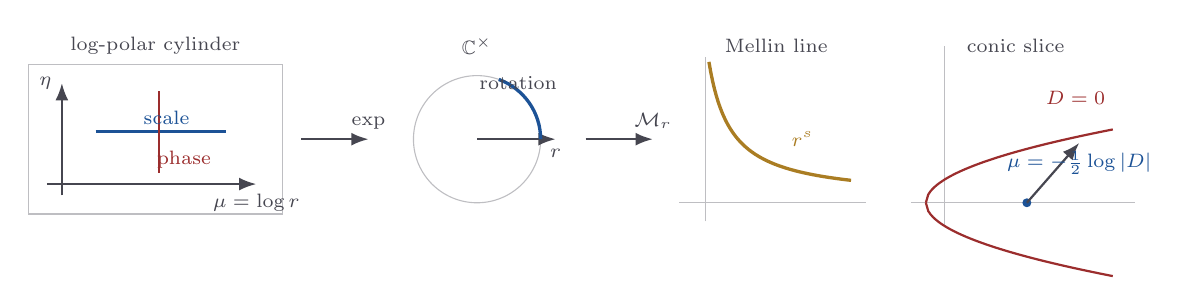
\begin{tikzpicture}[scale=0.95]
  \begin{scope}
    \draw[faint] (0,0) rectangle (3.4,2.0);
    \draw[arrow] (0.25,0.4) -- (3.05,0.4) node[ann,below] {$\mu=\log r$};
    \draw[arrow] (0.45,0.25) -- (0.45,1.75) node[ann,left] {$\eta$};
    \draw[hlt] (0.9,1.1) -- (2.65,1.1);
    \draw[deg] (1.75,0.55) -- (1.75,1.65);
    \node[ann] at (1.7,2.25) {log-polar cylinder};
    \node[ann,dblue] at (1.85,1.28) {scale};
    \node[ann,dred] at (2.08,0.72) {phase};
  \end{scope}
  \draw[arrow] (3.65,1.0) -- (4.55,1.0) node[ann,above] {$\exp$};
  \begin{scope}[xshift=5.0cm]
    \draw[faint] (1.0,1.0) circle (0.85);
    \draw[arrow] (1.0,1.0) -- (2.05,1.0) node[ann,below] {$r$};
    \draw[hlt] (1.85,1.0) arc (0:70:0.85);
    \node[ann] at (1.0,2.25) {$\C^\times$};
    \node[ann] at (1.55,1.75) {rotation};
  \end{scope}
  \draw[arrow] (7.45,1.0) -- (8.35,1.0) node[ann,above] {$\mathcal M_r$};
  \begin{scope}[xshift=8.8cm]
    \draw[faint] (-0.1,0.15) -- (2.4,0.15);
    \draw[faint] (0.25,-0.1) -- (0.25,2.1);
    \draw[gold,domain=0.3:2.2,samples=80] plot (\x,{0.2+0.55/(\x)});
    \node[ann] at (1.2,2.25) {Mellin line};
    \node[ann,dgold] at (1.55,1.0) {$r^s$};
  \end{scope}
  \begin{scope}[xshift=12.0cm]
    \draw[faint] (-0.2,0.15) -- (2.8,0.15);
    \draw[faint] (0.25,-0.15) -- (0.25,2.25);
    \draw[deg,domain=0:2.5,samples=80] plot (\x,{0.15+0.62*sqrt(\x)});
    \draw[deg,domain=0:2.5,samples=80] plot (\x,{0.15-0.62*sqrt(\x)});
    \fill[dblue] (1.35,0.15) circle (1.7pt);
    \draw[arrow] (1.35,0.15) -- (2.05,0.95);
    \node[ann] at (1.2,2.25) {conic slice};
    \node[ann,dred] at (2.0,1.55) {$D=0$};
    \node[ann,dblue] at (2.05,0.68) {$\mu=-\frac12\log|D|$};
  \end{scope}
\end{tikzpicture}
\caption{Scale--phase factorization in conic coordinates.  The
log-polar cylinder separates scale $\mu$ from phase $\eta$; complex
exponentiation returns dilation and rotation on $\C^\times$; the
Mellin transform diagonalizes scale; the conic discriminant
$D=\lambda^2-4$ supplies the logarithmic scale coordinate
$\mu=-\frac12\log|D|$.}
\label{fig:scale-phase-mellin}
\end{figure*}

Let $\mathsf R_\omega e^{im\eta}=e^{im\omega}e^{im\eta}$ be phase
rotation and let $\mathsf T_\mu$ be the scale semigroup coming from
radial Poisson continuation,
\[
  \mathsf T_\mu e^{im\eta}=e^{-\mu |m|}e^{im\eta}.
\]
Then the infinitesimal generator of scale is $-|D_\eta|$.  With the
normalization of this paper, $Q_{S^1}=\pi|D_\eta|$.

\begin{proposition}[scale--phase intertwiner]\label{prop:scale-phase}
Suppose $A$ is a positive self-adjoint translation-invariant operator
on $L^2_0(\T)$ whose heat semigroup intertwines conic scale
translation and phase rotation:
\[
  e^{-\mu A/\pi}\mathsf R_\omega e^{im\eta}
  =e^{-\mu |m|}e^{im\omega}e^{im\eta}
  \quad(m\in\mathbb Z\setminus\{0\}).
\]
Then $A=\pi|D_\eta|=Q_{S^1}$.  Equivalently, the
log-discriminant Hessian is the unique order-one positive generator
compatible with the Mellin scale coordinate and the angular Fourier
phase coordinate.
\end{proposition}

\begin{proof}
Translation invariance diagonalizes $A$ in the Fourier basis:
$Ae^{im\eta}=a_m e^{im\eta}$.  Comparing the scale multipliers in
the displayed intertwining identity gives
$e^{-\mu a_m/\pi}=e^{-\mu |m|}$ for every $\mu>0$, hence
$a_m=\pi|m|$.
\end{proof}

\subsection{Shape recovery from \texorpdfstring{$Q^2$}{Q2} and exact spectral area}

Here $Q^2$ means the full squared operator or matrix on mean-zero
boundary data, not merely the unordered list of eigenvalues.  Since
$Q_\Gamma$ is positive on constants removed, the squared operator
contains the same noiseless information:
\[
  Q_\Gamma=(Q_\Gamma^2)^{1/2}\quad\text{on }L^2_0(\Gamma).
\]
Thus a recovery pipeline may take $Q^2$ as its only operator input,
take the positive square root spectrally, recover the boundary
geometry from the resulting order-one operator, and compute area from
the recovered spectral boundary coefficients.

\begin{figure*}[t]
\centering
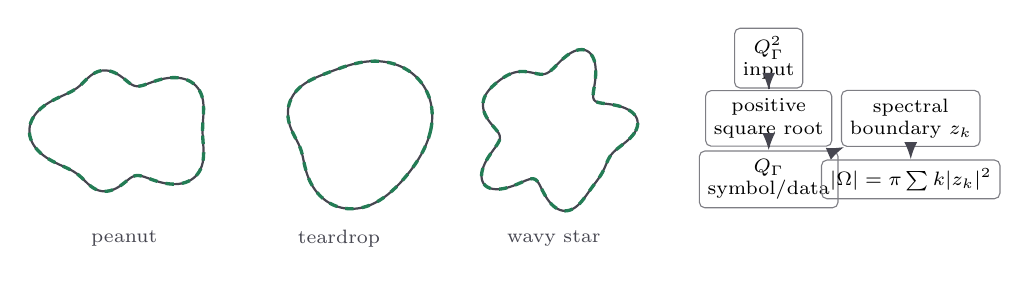
\begin{tikzpicture}[scale=0.88]
  \begin{scope}
    \draw[prim,domain=0:360,samples=180,smooth]
      plot ({(1+0.25*cos(2*\x)-0.12*cos(5*\x))*cos(\x)},
            {(1+0.25*cos(2*\x)-0.12*cos(5*\x))*sin(\x)});
    \draw[greenline,dashed,domain=0:360,samples=180,smooth]
      plot ({(1+0.25*cos(2*\x)-0.12*cos(5*\x))*cos(\x)},
            {(1+0.25*cos(2*\x)-0.12*cos(5*\x))*sin(\x)});
    \node[ann] at (0,-1.55) {peanut};
  \end{scope}
  \begin{scope}[xshift=3.1cm]
    \draw[prim,domain=0:360,samples=180,smooth]
      plot ({(1+0.32*cos(\x)+0.10*sin(3*\x))*cos(\x)},
            {(1+0.32*cos(\x)+0.10*sin(3*\x))*sin(\x)});
    \draw[greenline,dashed,domain=0:360,samples=180,smooth]
      plot ({(1+0.32*cos(\x)+0.10*sin(3*\x))*cos(\x)},
            {(1+0.32*cos(\x)+0.10*sin(3*\x))*sin(\x)});
    \node[ann] at (0,-1.55) {teardrop};
  \end{scope}
  \begin{scope}[xshift=6.2cm]
    \draw[prim,domain=0:360,samples=220,smooth]
      plot ({(1+0.18*cos(5*\x)+0.09*sin(7*\x))*cos(\x)},
            {(1+0.18*cos(5*\x)+0.09*sin(7*\x))*sin(\x)});
    \draw[greenline,dashed,domain=0:360,samples=220,smooth]
      plot ({(1+0.18*cos(5*\x)+0.09*sin(7*\x))*cos(\x)},
            {(1+0.18*cos(5*\x)+0.09*sin(7*\x))*sin(\x)});
    \node[ann] at (0,-1.55) {wavy star};
  \end{scope}
  \begin{scope}[xshift=9.3cm]
    \node[box] (a) at (0,1.05) {$Q_\Gamma^2$\\input};
    \node[box] (b) at (0,0.18) {positive\\square root};
    \node[box] (c) at (0,-0.70) {$Q_\Gamma$\\symbol/data};
    \node[box] (d) at (2.05,0.18) {spectral\\boundary $z_k$};
    \node[box] (e) at (2.05,-0.70) {$|\Omega|=\pi\sum k|z_k|^2$};
    \draw[arrow] (a) -- (b);
    \draw[arrow] (b) -- (c);
    \draw[arrow] (c) -- (d);
    \draw[arrow] (d) -- (e);
  \end{scope}
\end{tikzpicture}
\caption{Schematic \(Q^2\)-only recovery for hard non-round analytic
test shapes.  The gray curve is the target boundary and the
green dashed curve is the recovered spectral boundary in the noiseless
operator model.  The key point is that positivity makes \(Q\) the
unique square root of \(Q^2\) on mean-zero data; once the boundary is
represented spectrally, area is the exact Fourier sum
\eqref{eq:spectral-area}.}
\label{fig:q2-funky-recovery}
\end{figure*}

\begin{proposition}[\(Q^2\)-only recovery and area]\label{prop:q2-area}
Assume an analytic Jordan curve is recovered from the full operator
$Q_\Gamma^2$ in an arclength boundary representation, with constants
removed.  Then:
\begin{enumerate}
\item \(Q_\Gamma\) is determined uniquely by functional calculus as
\((Q_\Gamma^2)^{1/2}\).
\item In a general boundary parameter, the principal symbol of
\(Q_\Gamma\) fixes the arclength scale; in arclength form this
normalization is \(\pi|\xi|\).  The remaining lower-order part is the
operator data from which curvature-sensitive reconstruction terms must
be read.
\item If the recovered oriented boundary has complex Fourier series
\[
  z(\theta)=\sum_{k\in\mathbb Z}z_k e^{ik\theta},
  \qquad 0\le\theta<2\pi,
\]
then its signed area is computed spectrally by
\begin{equation}\label{eq:spectral-area}
  A_{\rm signed}(\Omega)
  =\frac12\int_0^{2\pi}\operatorname{Im}(\overline z\,z')\dd\theta
  =\pi\sum_{k\in\mathbb Z}k\,|z_k|^2 .
\end{equation}
For a trigonometric-polynomial boundary this formula is exact as a
finite sum; for analytic boundaries it converges exponentially.
\end{enumerate}
\end{proposition}

\begin{proof}
The first statement is the spectral theorem for a positive
self-adjoint operator.  The second is Theorem~\ref{thm:dtn} read in
reverse: the order-one symbol fixes arclength scale, while the
zeroth-order remainder is where curvature enters.  For the area
formula, write \(z'=\sum_k ikz_ke^{ik\theta}\) and integrate
\(\overline z z'\).  Orthogonality leaves
\(\int_0^{2\pi}\overline z z'\dd\theta
=2\pi i\sum_k k|z_k|^2\); taking one half of the imaginary part gives
\eqref{eq:spectral-area}.
\end{proof}

\subsection{Non-circulant hard-shape examples}

To make the preceding proposition concrete, consider analytic
star-shaped boundaries
\[
  \begin{aligned}
  z(\theta)&=r(\theta)e^{i\theta},\\
  r(\theta)&=1+\sum_p\bigl(a_p\cos(p\theta)+b_p\sin(p\theta)\bigr).
  \end{aligned}
\]
These are not circulant examples: the sampled chord matrix
\[
  A_{ij}=|z(\theta_i)-z(\theta_j)|^{-2}\qquad (i\ne j),
  \qquad A_{ii}=0,
\]
does not depend only on \(i-j\).  We measure this by the relative
distance to the best cyclic-diagonal average
\[
  d_{\rm circ}
  =\frac{\|A-\Pi_{\rm circ}A\|_F}{\|A\|_F},
\]
where \(\Pi_{\rm circ}\) projects a matrix to the nearest circulant
matrix by averaging each cyclic diagonal.  The circle has
\(d_{\rm circ}=0\); the examples below are dense, genuinely
non-circulant tests.

For these finite Fourier boundaries, the spectral area is exactly
\[
  A_{\rm spec}=\pi\sum_k k|z_k|^2
  =\pi\left(1+\frac12\sum_p(a_p^2+b_p^2)\right),
\]
where the second equality follows after substituting
\(z=r e^{i\theta}\).  Table~\ref{tab:hard-shape-area} reports the
area computed from the Fourier coefficients and verifies it against a
high-order shoelace computation on \(2^{14}\) boundary samples.

\begin{table*}[t]
\centering
\caption{Non-circulant hard-shape examples.  The non-circulant defect
uses \(n=256\) samples of the off-diagonal chord matrix.  The area is
computed spectrally from \(\pi\sum k|z_k|^2\); the final column is the
absolute difference from a \(2^{14}\)-point shoelace check.}
\label{tab:hard-shape-area}
\scriptsize
\setlength{\tabcolsep}{2pt}
\begin{tabular}{lp{0.43\textwidth}rrrr}
\toprule
shape & \(r(\theta)-1\) & \(r_{\min}\) & \(d_{\rm circ}\) &
\(A_{\rm spec}\) & shoelace diff.\\
\midrule
peanut
& \(0.32\cos2\theta-0.10\cos5\theta\)
& \(0.6210\) & \(0.4887\) & \(3.3181501607\) & \(1.6{\times}10^{-7}\)\\
teardrop
& \(0.35\cos\theta+0.12\sin3\theta-0.06\cos4\theta\)
& \(0.5465\) & \(0.5159\) & \(3.3622895375\) & \(1.2{\times}10^{-7}\)\\
wavy star
& \(0.18\cos5\theta+0.09\sin7\theta+0.06\cos11\theta\)
& \(0.6944\) & \(0.4440\) & \(3.2108647716\) & \(2.7{\times}10^{-7}\)\\
asymmetric gear
& \(0.24\cos3\theta-0.18\sin4\theta+0.10\cos8\theta-0.06\sin9\theta\)
& \(0.4427\) & \(0.5684\) & \(3.3043271530\) & \(3.1{\times}10^{-7}\)\\
three-lobed
& \(-0.22\sin2\theta+0.31\cos3\theta+0.08\sin6\theta\)
& \(0.4437\) & \(0.6327\) & \(3.3786258193\) & \(2.3{\times}10^{-7}\)\\
\bottomrule
\end{tabular}
\end{table*}

These examples are useful because they separate three notions that
coincide on the circle.  The chord matrix is no longer circulant, so
FFT diagonalization is not available directly.  The operator is still
the same positive order-one \(Q_\Gamma\), so \(Q_\Gamma^2\) still
determines \(Q_\Gamma\) by the positive square root.  Once the
boundary is recovered in Fourier form, the area is not measured by a
mesh rule; it is the spectral invariant \eqref{eq:spectral-area}.

\section{Discussion and Limitations}

The log-discriminant Hessian provides a compact algebraic route to a
classical analytic object.  On roots of unity it is exactly
diagonalizable; after arclength weighting it converges to
$\pi|D|$; on a smooth curve it is $\pi\Lambda_\Gamma$ modulo
zeroth-order terms.  This explains why the same inverse-square kernel
appears in three places: the Hessian of $\log|\Delta|$, the
hypersingular boundary operator, and the local profile of
near-singular quadrature.

Several points are deliberately scoped.  The closed-form spectrum and
FFT calculus are circle-specific.  On nonuniform Fekete nodes or
general analytic curves, $Q_{\Gamma,n}$ is dense and its fast
application requires the same fast-multipole or hierarchical machinery
used for other boundary integral operators.  The minimax theorem
requires analyticity; finite smoothness gives algebraic widths, and
the sharp $C^k$ analogue of \eqref{eq:minimax} is not included here.
Finally, the discriminant-cone and inverse-spectral interpretations
are useful geometric readings of the same operator but are not needed
for the SIAM numerical-analysis core presented above.

\appendix

\section{Details for the Spectral Tail}

This appendix expands the proof of Theorem~\ref{thm:zeta-tail}.  The
point is not the novelty of the contour calculation; it is the way the
finite polynomial spectrum separates into an interior Riemann-sum
term and two endpoint tails.

Put $x_k=k/n$.  Since
\[
  \frac{k(n-k)}{n}=n\,x_k(1-x_k),
\]
we may write
\[
  S_n(s)=n^{-s}\sum_{k=1}^{n-1}
  \bigl(x_k(1-x_k)\bigr)^{-s}.
\]
The beta term is the corresponding continuum contribution
\[
  n^{1-s}B(1-s,1-s)
  =n^{1-s}\int_0^1 \bigl(x(1-x)\bigr)^{-s}\dd x .
\]
The only non-smooth points of the integrand are the two endpoints.
Choose $M$ with $1\ll M\ll n$ and split the sum into the two endpoint
pieces and the middle.  At the left endpoint,
\[
  \begin{aligned}
  \bigl(k(1-k/n)\bigr)^{-s}
  &=k^{-s}\left(1-\frac{k}{n}\right)^{-s}\\
  &=k^{-s}+O_K(k^{1-\operatorname{Re}s}/n).
  \end{aligned}
\]
uniformly for $s$ in a fixed compact set $K$ away from the positive
integers; the right endpoint gives the same contribution.  On the
middle interval Euler--Maclaurin applies to
\((x(1-x))^{-s}\) with its endpoint pieces removed.  In the initial
strip \(0<\operatorname{Re}s<1\), this gives
\[
  \begin{aligned}
  &S_n(s)-n^{1-s}B(1-s,1-s)\\
  &\quad=
  2\left[
    \sum_{k=1}^{M}k^{-s}
    -\frac{M^{1-s}}{1-s}
  \right]\\
  &\qquad+O_K(M^{-\operatorname{Re}s})
       +O_K(M^2/n).
  \end{aligned}
\]
Letting first $n\to\infty$ and then $M\to\infty$ gives the standard
Euler--Maclaurin continuation
\[
  \zeta(s)=
  \lim_{M\to\infty}
  \left[
    \sum_{k=1}^{M}k^{-s}
    -\frac{M^{1-s}}{1-s}
  \right],
\]
and therefore the two endpoint tails contribute \(2\zeta(s)\) in the
strip.  For a general compact \(K\subset
\C\setminus\mathbb Z_{\ge1}\), repeat the same endpoint split with a
fixed number of Euler--Maclaurin subtractions large enough for \(K\).
The subtracted endpoint polynomials are exactly the meromorphic
continuation terms for \(\zeta(s)\), and the remaining middle
Riemann-sum error is \(O_K(n^{-1})\).  At $s=0$ the identity is finite
and direct:
$S_n(0)=n-1$, $nB(1,1)=n$, hence $T_n(0)=-1$.

\section{Details for the Bridge Estimate}

We collect the local estimates used in Theorem~\ref{thm:bridge}.  Let
$x$ have closest boundary point $s_0$, and introduce Frenet
coordinates with $s_0=0$ and $x=(0,\delta)$.  For
$\gamma(s)=(s,\kappa_0s^2/2)+O(s^3)$,
\[
  |x-\gamma(s)|^2=s^2+\delta^2-\kappa_0\delta s^2+O(s^4+\delta s^3).
\]
Thus, on $|s|<c$,
\begin{equation}\label{eq:app-local-log}
  \log|x-\gamma(s)|
  =
  \frac12\log(s^2+\delta^2)+\psi(s,\delta),
\end{equation}
where $\psi$ is $C^2$ and its norm is bounded by curvature and reach
constants.  The first term gives the universal profile; the second
is the smooth local remainder.

\begin{lemma}[inverse-square localization]\label{lem:app-Qdelta}
If $\sigma$ is continuous and nonzero at $s_0$, then
\[
  \int_\Gamma\frac{|\sigma(t)|}{|x-\gamma(t)|^2}\dd t
  =
  \frac{\pi|\sigma(s_0)|}{\delta}+O(1),
  \qquad \delta\downarrow0.
\]
\end{lemma}

\begin{proof}
Split the integral into $|s|<c$ and its complement.  The complement
is bounded.  In the local part use
$|x-\gamma(s)|^2=s^2+\delta^2+O(\delta s^2+s^4)$ and
$\sigma(s)=\sigma(s_0)+O(s)$.  The odd term integrates to zero at
principal order, and
$\int_{-c}^c(s^2+\delta^2)^{-1}\dd s
=2\delta^{-1}\arctan(c/\delta)=\pi\delta^{-1}+O(1)$.
\end{proof}

\begin{lemma}[profile expansions]\label{lem:app-profile-exp}
The function
$\mathcal M(\rho,\beta)=\operatorname{Re}\log(1-e^{-2\pi\rho+2\pi i\beta})$
satisfies
\[
\mathcal M(\rho,\beta)
=-e^{-2\pi\rho}\cos(2\pi\beta)+O(e^{-4\pi\rho})
\quad(\rho\to\infty),
\]
\[
\begin{aligned}
\mathcal M(0,\beta)&=\log|2\sin(\pi\beta)|\quad(\beta\ne0),\\
\mathcal M(\rho,0)&=\log(2\pi\rho)+O(\rho).
\end{aligned}
\]
\end{lemma}

These elementary expansions are the practical content of the
Quadrature--Curvature Law.  In the resolved regime $\rho\gg1$, the
local term is exponentially small and is indistinguishable from the
classical strip estimate.  In the underresolved regime $\rho=O(1)$,
the local term is $O(h)$ and stops improving exponentially with
$\delta$ at fixed $n$.  When the target is node-aligned
($\beta=0$), the logarithmic singularity is visible; when it is
halfway between nodes, the leading sign and amplitude differ.

The Donaldson--Elliott representation gives the complementary bulk
estimate.  For an analytic $L$-periodic function $f$,
\[
  I[f]-I_n[f]
  =\frac{1}{2\pi i}\int_C f(z)
  \frac{1}{e^{2\pi iz/h}-1}\dd z.
\]
If $C$ is moved to height $a>0$, the denominator contributes
$e^{-2\pi a/h}$ and the integral is controlled by the supremum of
$f$ on that contour.  When $f$ is the smooth part in
\eqref{eq:app-local-log}, the contour can be moved until it meets the
nearest analytic obstruction, giving the bulk channel in
\eqref{eq:bridge}.  When $f$ is the local logarithm, the contour
cannot cross the branch point at height $\delta$; the keyhole around
that branch point gives precisely the Poisson profile.

\section{Implementation Notes}

The circle algorithm used in the experiments is short enough to state
explicitly.
\begin{enumerate}
\item Given node values $u_j$, compute $\widehat u=F_nu$ by FFT.
\item Multiply each mode by
$\lambda_m=m(n-m)/2$, or by the requested scalar
$\varphi(\lambda_m)$ for a functional calculus call.
\item Set the zero mode to zero for $Q_n$ or for the inverse on
$\one^\perp$; for a heat kernel or resolvent use the requested
zero-mode value.
\item Apply the inverse FFT.
\end{enumerate}
The row-sum nullspace is exact in spectral form because
$\lambda_0=0$ is assigned explicitly.  For general curves the same
operator is assembled by \eqref{eq:nystrom}.  The diagonal is never
quadrature-evaluated; it is set by row-sum completion:
\[
  (Q_{\Gamma,n})_{ii}=\sum_{j\ne i}
  \frac{w_j}{|\gamma(s_i)-\gamma(s_j)|^2}.
\]
This is the discrete analogue of subtracting $f(t)$ from $f(s)$ in
\eqref{eq:Q-cont}; it is also the step that preserves the constant
nullspace.

For nonuniform nodes, the operator is naturally symmetric in the
weighted inner product
$\ip{u}{v}_w=\sum_i w_i\overline{u_i}v_i$.  If a Euclidean symmetric
matrix is desired, use
\[
  \widetilde Q_{\Gamma,n}
  =D_w^{1/2}Q_{\Gamma,n}D_w^{-1/2}.
\]
This similarity transform leaves the spectrum unchanged and restores
standard symmetric eigensolvers.  Fast application away from the
circle is not an FFT problem; it is a standard kernel-summation
problem with inverse-square kernel and can be accelerated by FMM,
$H$-matrices, or local panel compression.

\section{Additional Scope Notes}

The statement $Q_\Gamma=\pi\Lambda_\Gamma+K_0$ is stable under smooth
changes of parametrization when $Q_\Gamma$ is written in arclength
measure.  If a non-arclength parameter $t$ is used, the weights and
the kernel must include the speed $|\gamma'(t)|$; otherwise the
principal symbol is conjugated by the density of the parameter and
the constant $\pi$ is obscured.

The analytic minimax theorem is also sensitive to coordinates.  The
quantity $\delta_\Phi(x)$ is not Euclidean distance.  Near a smooth
point the two are comparable through the conformal Jacobian, but
global geometry enters the constants.  This is why the ellipse tests
show a rate fixed by conformal target distance and a prefactor varying
with the ellipse modulus.

The finite-smoothness regime remains open in the same clean form.  A
$C^k$ density has algebraic Fourier decay, so the rate cannot be
\eqref{eq:minimax}.  The near-singular bridge still applies to any
fixed rule, and $\mathcal Q(x)$ still identifies the dangerous local
scale, but the optimal information-based width is a different
problem.

\begin{thebibliography}{99}

\bibitem{AndrievskiiBlatt2002}
V.~V. Andrievskii and H.-P. Blatt,
\emph{Discrepancy of Signed Measures and Polynomial Approximation},
Springer, New York, 2002.

\bibitem{DonaldsonElliott1972}
A.~B. Donaldson and D. Elliott,
A unified approach to quadrature rules with asymptotic estimates of
their remainders,
\emph{SIAM J. Numer. Anal.}, 9 (1972), pp. 573--602.

\bibitem{HelsingOjala2008}
J. Helsing and R. Ojala,
On the evaluation of layer potentials close to their sources,
\emph{J. Comput. Phys.}, 227 (2008), pp. 2899--2921.

\bibitem{Hormander1985}
L. H{\"o}rmander,
\emph{The Analysis of Linear Partial Differential Operators III},
Springer, Berlin, 1985.

\bibitem{KlintebergTornberg2017}
L. af Klinteberg and A.-K. Tornberg,
Error estimation for quadrature by expansion in layer potential
evaluation,
\emph{Adv. Comput. Math.}, 43 (2017), pp. 195--234.

\bibitem{Kloeckner2013}
A. Kl{\"o}ckner, A. Barnett, L. Greengard, and M. O'Neil,
Quadrature by expansion: A new method for the evaluation of layer
potentials,
\emph{J. Comput. Phys.}, 252 (2013), pp. 332--349.

\bibitem{Maue1949}
A.-W. Maue,
Zur Formulierung eines allgemeinen Beugungsproblems durch eine
Integralgleichung,
\emph{Z. Phys.}, 126 (1949), pp. 601--618.

\bibitem{McLean2000}
W. McLean,
\emph{Strongly Elliptic Systems and Boundary Integral Equations},
Cambridge University Press, Cambridge, 2000.

\bibitem{NovakWozniakowski2008}
E. Novak and H. Wo{\'z}niakowski,
\emph{Tractability of Multivariate Problems. Volume I: Linear
Information},
European Mathematical Society, Z{\"u}rich, 2008.

\bibitem{Pinkus1985}
A. Pinkus,
\emph{$n$-Widths in Approximation Theory},
Springer, Berlin, 1985.

\bibitem{SaffTotik1997}
E.~B. Saff and V. Totik,
\emph{Logarithmic Potentials with External Fields},
Springer, Berlin, 1997.

\bibitem{SauterSchwab2011}
S.~A. Sauter and C. Schwab,
\emph{Boundary Element Methods},
Springer, Berlin, 2011.

\bibitem{TW2014}
L.~N. Trefethen and J.~A.~C. Weideman,
The exponentially convergent trapezoidal rule,
\emph{SIAM Rev.}, 56 (2014), pp. 385--458.

\end{thebibliography}

\end{document}
